%%This is a very basic article template.
%%There is just one section and two subsections.
\documentclass[a4paper]{article}

\usepackage[utf8]{inputenc}
\usepackage[T1]{fontenc}
\usepackage[francais]{babel}
\usepackage[colorlinks=true]{hyperref}
\usepackage{verbatim} % adds environment for commenting out blocks of text & for
% better verbatim

\usepackage{wrapfig}
\usepackage{graphicx}

\usepackage{xcolor}
\usepackage{listings}
\usepackage{courier}
\lstset{
         basicstyle=\footnotesize\ttfamily, % Standardschrift
         numbers=left,               % Ort der Zeilennummern
         numberstyle=\tiny,          % Stil der Zeilennummern
         numbersep=5pt,              % Abstand der Nummern zum Text
         tabsize=2,                  % Groesse von Tabs
         extendedchars=true,         %
         breaklines=true,            % Zeilen werden Umgebrochen
         keywordstyle=\color{red},
    		frame=b,
         stringstyle=\color{white}\ttfamily, % Farbe der String
         showspaces=false,           % Leerzeichen anzeigen ?
         showtabs=false,             % Tabs anzeigen ?
         xleftmargin=17pt,
         framexleftmargin=17pt,
         framexrightmargin=5pt,
         framexbottommargin=4pt,
         %backgroundcolor=\color{lightgray},
         showstringspaces=false      % Leerzeichen in Strings anzeigen ?        
 }
\lstloadlanguages{% Check Dokumentation for further languages ...
         %[Visual]Basic
         %Pascal
         %C
         %C++
         XML
         %HTML
         %Java
 }
\usepackage{caption}
\DeclareCaptionFont{blue}{\color{blue}} 
\captionsetup[lstlisting]{singlelinecheck=false, labelfont={blue}, textfont={blue}}
\DeclareCaptionFont{white}{\color{white}}
\DeclareCaptionFormat{listing}{\colorbox[cmyk]{0.43, 0.35, 0.35,0.01}{\parbox{\textwidth}{\hspace{15pt}#1#2#3}}}
\captionsetup[lstlisting]{format=listing,labelfont=white,textfont=white, singlelinecheck=false, margin=0pt, font={bf,footnotesize}}

\title{LodPaddle et OpenDataWrapper - HOW TO}
\author{Sébastien CHENAIS}
\date{juin 2013}

\begin{document}
\maketitle
\newpage

\tableofcontents %% produire à cet endroit la table des matièree					
\newpage

\section{LodPaddle et le web sémantique}
\subsection{Présentation de LodPaddle}

LodPaddle est un projet porté par Hala Skaf-Molli du LINA\footnote{Laboratoire
d'Informatique de Nantes Atlantique} et fait écho au projet Européen
Lod2\footnote{LOD2:
\href{http://lod2.eu/WikiArticle/Project.html}{http://lod2.eu/WikiArticle/Project.html}}
qui a pour but de faciliter la production et l'exploitation de données au format
spécifique du web sémantique. Pour ce faire, Lod2 nous propose une suite
d'outils qui permettent l'extraction et la conversion de donnée, leur mise en
ligne, les liens entre les différentes entités, leur enrichissement \ldots{}

Depuis quelques temps, le conseil général de la Loire-Atlantique, la région Pays
de la Loire et la ville de Nantes on ouvert un pole Open Data dans leur
département. Actuellement composé de 422 jeux de données sur des sujets variés
comme les écoles, les loisirs, les subventions, les transports \ldots{}, ces
données gagneraient énormément à être sémantifiées.

Le projet LodPaddle s'est donc associé aux acteurs du site
\href{http://data.paysdelaloire.fr}{data.paysdelaloire.fr} afin de sémantifier
leurs données, de permettre aux utilisateurs et développeurs de récupérer les
données au format RDF \footnote{Ressource Description Framework} ou d'interroger
directement un \begin{itshape}SPARQL Endpoint \footnote{Serveur web comprenant
le langage de requête SPARQL}\end{itshape} et de développer une application
pilote montrant que les données sémantifiées gagnent en valeur ajoutée.

\subsection{Qu'est ce que le web sémantique}

Aussi appelé web 3.0 ou web des données, le web sémantique est une évolution du
web que nous connaissons. Actuellement, énormément d'information est dispersé
sur la toile, comme sur wikipédia par exemple, mais il est difficile de
récupérer la bonne information rapidement. Par exemple, vous cherchez la liste
des capitales mondiale, vous allez faire une requête sur votre moteur de
recherche préféré, chercher une page qui pourrait éventuellement proposer la
solution puis chercher dans la page choisie la probable information. Et celà est
vrai uniquement si une personne a crée cette liste au préalable.

Dans le domaine du web sémantique, la réponse serait instantanément une liste
des capitales mondiales, au format texte, exploitable par un humain et une
machine.

\begin{lstlisting}[caption=Requête SPARQL récupérant la liste des capitales
mondiales, language=SPARQL]
select distinct ?nom where {
	?pays prop-fr:capitale ?capitale.
	?pays rdf:type dbpedia-owl:Country.
	?capitale prop-fr:nom ?nom .
}
\end{lstlisting}

Le résultat de cette requête donnerait une liste comme celle
présentée en \begin{textsc}figure-\ref{cap} \end{textsc}.

\begin{figure}[h]
    \centering
    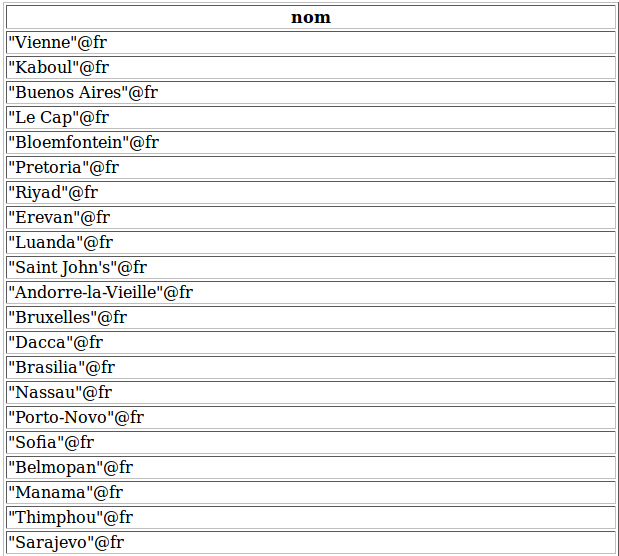
\includegraphics[scale=0.70]{img/capitales.png}
    \caption{\label{cap} Liste des capitales mondiales}
\end{figure}

\subsection{Le format Ressource Description Framework (RDF)}

Pour arriver au résultat précédent, nous avons besoin d'une syntaxe particulière
permettant de décrire les données sous forme d'objet manipulables: Le RDF. Ce
dernier fonctionne par triple de la forme Sujet - Predicat - Objet. Par exemple,
le sujet \og{} France \fg{} , le prédicat \og{} a pour capitale \fg{} et l'objet
\og{} Paris \fg{}. Avec ce format, on se rends compte qu'on peut simplement
demander une partie de ce triple en résultat; par exemple, donne moi tous les
triples qui ont pour sujet \og{} Paris \fg{}.


\subsection{Le Linked Open Data}

La force du web sémantique par rapport au stockage classique des donnée par base
de donnée, tableur et autres, vient du fait qu le sujet est identifié de façon
unique sur le web. Ainsi, si une autre personne que vous a crée ce même sujet,
vos données respectives voint pouvoir s'additionner: on appelle cela lier les
données. Lorsque l'on effectue une recherche sur le sujet, vos informations,
ainsi que toutes les informations produites par d'autres personnes concernant ce
sujet, sont donc disponible.

\section{Open Data Wrapper}

L'Open Data Wrapper est un outils développé en JAVA permettant la conversion
automatique des données de data.paysdelaloire.fr en données sémantifiées. Les
données sont récupérées automatiquement du site à travers leur API dans la
mesure du possible.

\subsection{Utilisation}

Lancez Open Data Wrapper. Après un léger temps de chargement, l'application vous
demande ce que vous souhaitez faire. Les propositions sont:
\begin{itemize}
\item lister les sources de donnée
\item convertir une source de donnée au format N3
\item convertir toutes les sources de donnée au format N3
\item convertir une source de donnée au format XML/RDF
\item convertir toutes les sources de donnée au format XML/RDF
\item quitter
\end{itemize}

Après selection d'une option, le traitement s'effectue.

\subsubsection{Les proxies}

Dans beaucoup d'organisation, le réseau est protégé par un proxy. Open Data
Wrapper est configurable pour utiliser des proxies. Pour ce faire, crée un
fichier proxy.pwd à la racine de votre compte (/home/utilisateur pour Linux,
C:/documents and setting/utilisateur pour Windows). Ce fichier comportera les
lignes suivantes:

\begin{lstlisting}[caption=Fichier de configuration des proxys proxy.pwd]
	proxyHost = url.du.proxy
	proxyPort = 3128 (port du proxy)
	authUser = nom d'utilisateur (vide si pas d'indentification)
	authPassword = mot de passe
\end{lstlisting}

L'authentification retenu par Open Data Wrapper est de type BASIC. Si vous avez
besoin de changer cela (NTLM par exemple), il vous faudra modifier le code.

\subsection{Développement}

Au cours du temps, les jeux de données vont s'enrichir et augmenter en nombre.
Voici la procédure pour ajouter une nouvelle source de donnée

\subsubsection{dataSources.xml}

Ce fichier contient toutes les informations necessaires à la conversion d'une
source de donnée.

\begin{lstlisting}[caption=Extrait de dataSources.xml, language=XML]
<source>
	<nom>Hotel</nom>
	<api>true</api>
	<apiurl>
		http://data.paysdelaloire.fr/api/publication/22440002800011_CG44_TOU_04815/hotels_STBL/content?format=xml
	</apiurl>
	<file>false</file>
	<filepath>null</filepath>
	<mappingFile>null</mappingFile>
	<xsltFile>ressources/hotel/hotelSaxon.xslt</xsltFile>
	<format>XML</format>
	<outputTtlFile>ressources/output/ttl/Hotel.n3</outputTtlFile>
	<outputXmlFile>ressources/output/rdf-xml/Hotel.rdf</outputXmlFile>
</source>
\end{lstlisting}

Pour ajouter une nouvelles source, il vous faut créer un nouveau n\oe{}ud
<source></source> puis ajouter les balises suivantes:
\\

\begin{itemize}
  \item{<nom>}: le nom de la nouvelle source.
  \item{<api>}: true si la source existe sur l'API, false sinon.
  \item{<apiurl}: l'URL API de la source. Ne sera lu uniquement si api vaut
  true. null si aucune url.
  \item{<file>}: true si la source existe localement, false sinon. Si API vaut
  true, cette valeur n'est pas prise en compte.
  \item{<filepath>}: le chemin du fichier ou null sinon.
  \item{<mappingFile>}: le chemin du fichier de mapping dans le cas de fichier
  source spécifique. Pas utilisé encore.
  \item{<xsltFile>}: chemin vers le fichier de transformation XSL ou XSLT.
  \item{<format>}: format du fichier. XML uniquement pour le moment (CSV
  rapidement).
  \item{<outputTtlFile>}: le chemin du fichier turtle en sortie.
  \item{<outputXmlFile>}: le chemin du fichier XML/RDF en sortie.
\end{itemize}

Votre source est ainsi ajoutée à Open Data Wrapper.

\subsubsection{ajout alternatif de source}

Si la modification du XML est fastidieuse ou que vous avez une grande liste de
dataset à ajouter, vous pouvez utiliser la fonction d'ajout de source. Pour ce
faire, créez un fichier nommé \textbf{import.odw} à la racine de votre compte
personel (\$home). Dans ce fichier la syntaxe d'ajout est la suivante: 

\begin{lstlisting}[caption=syntaxe import.odw, language=XML]
nom_du_dataset = http://url_de_l_api.com
\end{lstlisting}

Les restrictions liées à cette fonction sont les suivantes:

\begin{itemize}
  \item impossible d'importer autre chose que des fichiers XML par API
  \item le nom doit être composer uniquement de caractères alphanumériques et le
  caractère \_
  \item l'url de l'api ne comprend pas d'information de filtre ou de format
\end{itemize}

\subsubsection{mapping.properties}

Pour les données contactée par API, le format du fichier récupéré est de l'XML.
Sa transformation en RDF se fait à l'aide d'une feuille de transformation XSL.
Ce fichier est généré automatiquement par open Data Wrapper, en fonction du nom
des balises XML. Attention, il faut que chaque nom de balise correspondent à une
seule et uniquement une seule signification. De plus, le XML doit absolument
avoir une balise dont le vocabulaire correspondant est traduit en
\textbf{rdf:foaf}. Open Data Wrapper va prendre ses informations dans le
fichier mapping.properties, lire le nom de la balise, trouver le correspondant
RDF et génère un bloc de XSL. Si le nom de la balise n'est pas trouvé, un
message s'affiche et le fichier mapping.properties est mis à jour avec une
valeur par défaut. Vous devrez modifier cette valeur par la suite, pour lui
attribuer un réel sens.

\end{document}
